\documentclass[tikz,varwidth=30cm, multi=page]{standalone}
\usepackage{float}              % [H]
\usepackage{graphicx}           % (pdf, png, jpg, eps)
\usepackage{pgfplots}
\usepackage{siunitx}
\usepackage{currfile}
\usepackage{ifthen}
\usepackage{tikz}
\usetikzlibrary{calc}
\usepackage{pgfplots}
\usepackage{pgfplotstable}
\pgfplotsset{compat=1.17}
\usepgfplotslibrary{colorbrewer}
\usepgfplotslibrary{statistics}
% 
% \usetikzlibrary{external}
% \tikzexternalize[prefix=./output/tmp/]
% 
\def\datapath{output/cube_2pop_stat_0/time_evolve}
% 
\def\height{22.37076cm} %22.37076cm/5
\def\width{13.87303cm} %13.87303cm,
% 
\begin{document}
% 
\foreach \name in {times,overlaps,num_objs,num_col_objs}{
\begin{tikzpicture}[trim left=-10pt, trim axis right, baseline]
]
\begin{axis}[%
   cycle list/Dark2,
   ]
   \foreach \r in {0.5}{
   \foreach \fl in {2.0}{
   \foreach \fr in {2.0}{
   % \foreach \r in {0.5, 1.0}{
   % \foreach \fl in {2.0, 8.0}{
   % \foreach \fr in {2.0, 8.0}{
    \addplot+[%
       width = \width,
       height = 0.5*\height,
       only marks, mark=*,
       mark size=0.5pt,
       error bars/.cd,
       error bar style={line width=0.5pt},
       error mark options={rotate=90,mark size=2pt, line width=0.5pt},
       y dir=both,y explicit] table[
        x={steps_mean}, y={\name_mean}, y error=\name_std, col sep=comma,]
        {\datapath/cube_stat_time_evolve_r_\r_psi_0.5_fr_\fr_fl_\fl_.csv};
      %   \addlegendentryexpanded{$r=\r,f_l=\fl,f_r=\fr$}
   }}}
% 
\end{axis}
\end{tikzpicture}
}
% 
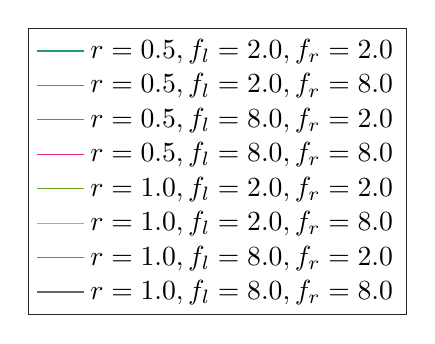
\begin{tikzpicture}[]
\begin{axis}[%
   legend cell align=left,
   % legend columns=2,
   % legend transposed=true,
   scale only axis, 
   width=1mm,
   hide axis,
   legend image post style={sharp plot},
   legend style={font=\vphantom{hg},draw=white!15!black,legend cell align=left, 
                 /tikz/every even column/.append style={column sep=1ex}},
   cycle list/Dark2,
   ]
   % 
   \foreach \r in {0.5, 1.0}{
   \foreach \fl in {2.0, 8.0}{
   \foreach \fr in {2.0, 8.0}{
         \addplot coordinates {(0,0)};
         \addlegendentryexpanded{$r=\r,f_l=\fl,f_r=\fr$}
   }}}
   % 
\end{axis}
\end{tikzpicture}
\end{document}
